\documentclass[11pt]{article}
\newcommand{\E}{\text{E}}
\usepackage{fullpage, amsmath, amsthm, graphicx, cite}
\usepackage[compact]{titlesec}

\setlength{\parindent}{0pt}
\newtheorem{thm}{Theorem}
\newtheorem{lem}[thm]{Lemma}
\newtheorem{prop}[thm]{Proposition}
\newtheorem*{cor}{Corollary}
\newtheorem*{rem}{Remark}
\newcommand{\vs}{\vspace{0.1cm}}
\date{}

{\makeatletter
 \gdef\subsection{\@ifnextchar*\subsection@star\subsection@normal}
 \gdef\subsection@normal#1{\refstepcounter{subsection}%
            \paragraph{\thesubsection\hbox{~~}#1.}}
 \gdef\subsection@star*#1{\paragraph{#1.}}}

\begin{document}
\title{The Lazy Engineer and Recommendation Subgraphs\thanks{This work was supported in part by an internship at BloomReach Inc.}}
\author{Arda Antikacioglu\thanks{Department of Mathematics, Carnegie
    Mellon University; aantikac@andrew.cmu.edu},
R. Ravi\thanks{Computer Science Department and Tepper School of Business, Carnegie Mellon
    University; ravi@cmu.edu}
~and
Srinath Sridhar\thanks{BloomReach Inc; srinath@bloomreach.com}}


\maketitle
\abstract

Recommendations are central to the utility of many of the popular websites such as YouTube,
Facebook and Quora, as well as the economic viability of e-commerce websites.
Such sites typically contain a set of recommendations on every product
page that enables visitors to easily navigate the website. Choosing
an appropriate set of recommendations at each page is one of the key
features of web relevance engines that have been commercially deployed 
at several retail sites.

Specifically in the case of BloomReach, an engine consisting of several independent
software components analyzes and optimizes its clients websites.
%Can cite ~\cite{WebRelevanceEngine} if needed.
This paper focuses on the structure optimizer component which
improves the website navigation experience so as to enable the discovery of previously
undiscovered content.

We begin the paper by formalizing the concept of recommendations that can be used to improve
the structure and discoverability of the website. We formulate this as a natural graph optimization
problem which, in its simplest case, reduces to a bipartite matching problem. In practice, solving these
matching problems requires super-linear time and is not scalable. Furthermore, implementing simple 
algorithms is paramount in practice because they are
significantly easier to maintain in a production software package. This motivated us to analyze 
three heuristic methods for solving the problem in increasing order of sophistication: 
a local random sampling algorithm,
a greedy algorithm and a partitioning algorithm that divides the edges into sets from which recommendations
are separately chosen.

We first theoretically analyze the performance of these three methods
on random graph models characterizing when each method will yield a solution of sufficient quality
and the parameter regimes when more sophistication is needed. 
We complement this by providing an empirical analysis
of these algorithms on simulated and real-world production data. Our
results confirm that it is not always necessary to implement complicated
algorithms in the real-world. Indeed, our results demonstrate that 
very good practical results 
can be obtained by using simple heuristics and 
backed by the confidence of concrete theoretical guarantees.

\iffalse

We formulate the problem of choosing the short list of recommendations from each page as one of choosing a subgraph of the candidate recommendation graph with the objective of maximizing the size of the recommended pages.

To inter-connect the website for efficient
traversal it is critical to choose a few recommendations on each
page from the list of all candidates.

In our formulation of the problem, the set of pages on the site is
divided into a few popular pages where surfers arrive and the
remaining large number of pages that should be recommended from the
popular pages. The natural bipartite graph of potential
recommendations is a candidate supergraph. Given the limited space to
display recommendations a subgraph that has bounded outdegree $c$ on the
popular pages must be chosen. Our goal is to maximize the number of
undiscovered pages that have indegree at least some target $a$. We introduce and study this
as the $(c, a)$-recommendation subgraph problem.

Solving such problems optimally at web-scale typically involves
writing distributed matching algorithms.  These can be incredibly hard
to implement, debug and scale effectively.  Instead, in this work, we
study the effectiveness of a lazy engineer solving the recommendation
subgraph problem. We investigate the cases when the candidate
supergraph is a random graph under two models: the fixed-degree model
where every node on the left has exactly $d$ random neighbors on the
right, as well as the standard Erd\"{o}s-Renyi model with expected
degree $d$ on the left side. We show that for most reasonable
parameters of the models, the lazy engineer would have found solutions
very close to optimal. We further show the conditions under which a
perfect recommendation subgraph, a generalization of perfect
matchings, exists. Lastly, to more realistically model web graphs, we
propose generalizations of the random graph models using topic
taxonomies, varying subgraph edge densities and edge weights that
capture the strength of recommendations. Surprisingly, the lazy
engineer would still have found near optimal solutions under different
realistic parameters, which we validate with some computational
testing on simulated models.
\fi 
\pagebreak

\setcounter{page}{1}
\begin{abstract}

Recommendations are central to the utility of many of the popular websites such
as YouTube, Facebook and Quora, as well as many e-commerce store websites.
Such sites usually have a large list of candidate pages that could serve as
recommendations from the current page based on relevance. To inter-connect
the website for efficient traversal it is critical to subselect a few
recommendations on each page from the list of all candidates.

%If every page is a
%node, these candidate recommendations can be denoted as directed
%edges. We introduce the recommendation subgraph problem which
%informally attempts to choose a subgraph of bounded
%outdegree (denoting the limited page space to display the
%ecommendations) such that the resulting graph and the website
%can be traversed `efficiently.'
%In a generalization of the problem, 
In our formulation of the problem, the set of pages on the site is divided into a few popular
pages where surfers arrive and the remaining large number of pages
that should be recommended from the popular pages. The natural
bipartite graph of potential recommendations is a candidate
supergraph. Given the limited space to display recommendations a
subgraph that has bounded outdegree $c$ on the popular pages must be
chosen. Our goal is to maximize the number of undiscovered pages that have
indegree at least $a$. We introduce this as the $(c,
a)$-recommendation subgraph problem. 
%Maximizing the number of pages that are recommended by at least two or more popular pages leads to a much harder problem.

%We describe our work in solving such recommendation subgraph problems in practice at web scale. 
To solve such problems optimally at web-scale graph sizes,
implementations would involve writing distributed matching
algorithms. Instead, in this work, we study the effectiveness of a
lazy engineer solving the recommendation subgraph problem.  We
investigate the cases when the candidate supergraph is a random graph
under two models: the fixed-degree model where every node on the left
has exactly $d$ random neighbors on the right, as well as the standard
Erd\"os-Renyi model with expected degree $d$ on the left side.  We
show that for most reasonable parameters of the models, the lazy
engineer would have found solutions very close to optimal. We further
show the conditions under which a perfect recommendation subgraph, a
generalization of perfect matchings, exists. Lastly, to more
realistically model web graphs we propose generalizations of the
random graph models using topic taxonomies, varying subgraph edge
densities and edge weights that simulate traffic patterns. Surprisingly, the lazy
engineer would still have found solutions near optimal under different parameters.

%We then extend the fixed-degree random graph model in many directions: one where the
%pages are situated in a natural hierarchical taxonomy (such as a topic ontology in Quora, or a product hierarchy in a store catalog), another where varying %densities are allowed between different subgraphs, and a third where the recommendation edges are weighted (typically according to the traffic that the %particular link is likely to generate) and the degree constraints are on the weighted degree. In all these cases, we identify conditions under which the lazy %engineer is very effective. We conclude with web-scale experimental results that motivate and validate our proposed models, as well as compare the %effectiveness of various heuristic methods that the lazy engineer would have then thought up in his freed up time.

\iffalse
In this paper, we study the problem of graph recommendations as
variants of bipartite matching problems. We consider the problem
of solving such matching problems in practice at web-scale. To achieve
this we introduce several models to simulate underlying input graph
structures. We then analyze the conditions under which a random sample
of edges using constant memory already suffices to be a
'good' recommendation algorithm as opposed the cases when we may consider
the more classical and involved linear memory polynomial time algorithms.
We also show how to select the number of recommendations per item while
building a website so that there exists a 'perfect' graph recommendation.
\fi

\end{abstract}

\section{Introduction}

One of the great benefits of the web as a useful source of hyperlinked
information comes from the careful choices made in crafting the recommendations
that link a given page to closely related pages. Even though this advantage was
identified well before the www was in place by Bush~\cite{Bush45}, it continues
to persist even in Web 2.0 systems that generate web pages of combined
information, where smooth navigation is enabled by carefully chosen
recommendations to closely related pages. Thus, the presence of recommendations
is an integral feature of several popular websites that are known to have high
user engagement as reflected in long user sessions. Examples range from 
entertainment sites like YouTube that recommend a set of videos on the right
for every video watched by a user, information sites like Quora that recommend
a set of related questions on every question page, to retail sites like Amazon
that recommend similar products on every product page. \vs

While recommendations are important, they are implemented typically by finding
related items to display at runtime. That is, when a user lands on an item the
recommendation systems decide online the set of other items to display. Such
systems have the problem that a global analysis of the performance of the
recommendations are hard. E.g., it is almost impossible to know if there is an
item that was not recommended by even one other item. As the number of
pages of a site grows, doing such a real-time computation becomes less ideal 
globally and might lead to deterioration in the link structure of the site.  This
motivates the strategy of solving the recommendation problem off-line, where we
pre-compute the set of recommendations for every item. Such a system can be
built in two stage: the first stage decides on candidate recommendations for each item
purely based on relevance and retrieves a large candidate set of $d$ items to
show [CITE A LOT OF PAPERS HERE FOR E.G.: Recommender systems in e-commerce
: http://dl.acm.org/citation.cfm?id=337035]. 
The second stages prunes it to $c < d$ items such that globally we ensure
that the resulting recommendation graph is `efficient' for traversal. For instance, we might want
to ensure that the resulting graph minimizes the number of items that was not
recommended by any other item. \vs

We can represent this notion of recommendations by using a directed graph. A
vertex is simply an item and a directed edge $(u, v)$ is a recommendation from
$u$ to $v$. Under this graph model for the above problem, if $c=1$ and we
require the chosen recommendation subgraph be strongly connected then our
problem reduces to Hamilton cycle, an NP-complete problem [CITE CLRS
OR SOMETHING HERE]. \vs

\subsection{Bipartite Recommendation Subgraphs}

We can generalize the above graph recommendation problem by using a directed
bipartite graph. Website owners might not be interested on all the items on
their site. We can use one partition $L$ (say, the one in the left) to represent
the set of items for which we are required  to suggest recommendations. We can
use the other partition $R$ (on the right) to represent the set of items that
are potentially recommended. Note that a single item can be represented in both
$L$ and $R$ if needed. We will use this representation to formulate all our
results. Now the input to the problem is this directed graph $G$ where each
vertex has $d$ recommendations (thanks to the first stage of the two-stage
recommendation back-end system described above). The output required is a
subgraph $G'$ where each vertex in $L$ has $c < d$ recommendations. The simplest
goal is to minimize the number of vertices that have in-degree less than an
integer quantity $a$. We call this the $(c, a)$-graph recommendation problem.
Note that if $a=c=1$ this is simply the problem of maximum bipartite matching
~\cite{LovaszPlummer} [OTHER CITATIONS?]. If $a=1$ and $c > 1$, this is still a degree-bounded
subgraph problem that can be converted to a polynomial-time solvable matching
problem called fractional matching [CITE FRACTIONAL MATCHING ON GRAPHS
PAPERS]\vs

Over the past few years, a subset of us have implemented such recommendation
subgraph algorithms in cutting-edge web-technology companies including Google,
Facebook and BloomReach. There are two key hurdles in making these
recommendation subgraph back-end systems practical. The first is that the method
used must be very simple to implement, debug and deploy. The second is that the
method must scale gracefully.  Matching algorithms require linear memory and
super-linear run-time neither of which scale well. Note that the Facebook graph
has over a billion vertices\cite{} and hundreds of billions of edges\cite{},
YouTube has XXX videos and YYY recommendations\cite{} etc. Even an e-commerce
website with 100M product pages and 10 recommendations per product would require
over 100GB in main memory to run these algorithms. Since using clusters of
single machines with such high memory is prohibitively expensive, MapReduce
\cite{} jobs are needed to solve these problems. However, such Map-reduce for
graph problems are notoriously hard and we are back to building a complicated
system. \vs

%Sri: Check out the para below and modify - add any figure/graph if you can justify these numbers here.
Our work with real-life web systems suggest that typical values for $c$ range
from 5 to 20, while the requirement $a$ is typically one, and sometimes slightly
larger in the range 2 to 5. The ratio of the size of undiscovered pages on the
right to the popular pages on the left is of the order of ten to hundred. It is
instructive to check the performance of the analyzed algorithms for these

Our work with real-life web systems suggest that typical values for $c$ range
from 5 to 20, while the requirement $a$ is typically one, and sometimes slightly
larger in the range 2 to 5. The ratio of the size of undiscovered pages on the
right to the popular pages on the left is of the order of ten to hundred. it is
instructive to check the performance of the analyzed algorithms for these
typical values of these parameters.

\subsection{Algorithms and Analyses}

{\bf The Lazy Engineer}
These reasons motivated the authors to investigate the ``lazy" approach of
choosing a very simple (any) set of recommendation to see if they would produce
near optimal solutions at least under realistic scenarios in practice. Our
initial goal was to find simple relationships between the parameters of the
problem and compute thresholds that dictate the need for different, more
sophisticated algorithms. In practice, this would immediately imply that a very
simple back-end system can be built in many cases without the need for a
complicated algorithm. If the thresholds provided by our analysis are
insufficient in quality, then the designer can consider implementing the
classical algorithms. \vs

{\bf Recommendation Graph Models} The setting for investigating the
effectiveness of the lazy engineer is provided by using a random graph
model for the recommendation supergraph. Since the lazy algorithm
involves choosing {\em any} set of $c$ recommendations, the natural
random graph model that permits analysis of this method is the {\em
  fixed-degree} model [CITE PAPERS FOR FIXED DEGREE] where every node
on the left has recommendations to a random subset of size exactly $d$
nodes in the right.

We study this model in Section~\ref{fixed-degree}. Our main result identifies
the range of parameters involving $c,a,l=|L|$ and $r =|R|$ where the lazy
algorithm is very effective. In addition to showing that it is a $(1-\frac1e)$-
approximation algorithm in expectation, we also get much better bounds for the
expected performance for a wide range of realistic parameters and also prove
high probability bounds on its performance. \vs

{\bf The Greedy Algorithm}
While the lazy algorithm chooses any set of $c$ recommendations, the natural
greedy algorithm will need some work: scanning the nodes on the right that must
be discovered, we look to see if there are $a$ neighbors from the left that have
not exhausted their bound of $c$ edges in the subgraph, and if so, use them to
add this node to the discovered set. We study this algorithm in Section
~\ref{greedy}. We show the easy result that Greedy gives a 
$\frac{1}{a+1}$-approximation, and also do an average case analysis. However, we
use the usual Erd\"os-Renyi model [CITE GNP PAPERS HERE] rather than the fixed-degree model for this
analysis.

In the subsequent Section~\ref{worst-vs-avg}, we compare and plot the worst-case
performance of Greedy against the average case expected performance of the random
or lazy algorithm, as a basis for our later computational comparisons in a
similar vein. \vs

{\bf Optimal Recommendation Subgraphs}
Finally we turn to the question of whether the maximum number of nodes allowed
by the degree constraints can be covered (at least $a$ times) by a recommendation
subgraph: we say that there is an perfect $(c,a)$-recommendation subgraph in this
case. Under the usual Erd\"os-Renyi model, we use existing results on the
existence of a perfect matching to characterize the edge probability over which
there exist such optimal recommendation subgraphs, by using a subset partitioning
method for the analysis. By relaxing the condition of optimality of matching (i.e.
perfect matchings) to disallowing short augmenting paths in these methods, we also
turn the above results into $(1-\epsilon)$-approximation algorithms trading off
the running time, for appropriately dense random graphs as before. \vs

\subsection{New Recommendation Graph Models}
The analysis of the various algorithms suggests that there may be more general
settings where the lazy and greedy algorithms perform well. We use our
experience in working with practical web systems to propose three such models
that generalize the fixed-degree model by taking into account (i) a natural
hierarchy in the organization of the pages, (ii) a partition of pages into
disjoint categories and varying density of connections between different
categories, and (iii) a weighting of the edges of the recommendation supergraph
based on the traffic generated along each of these links. \vs

{\bf A Hierarchical Model} 
Most information sources organize their pages according to a natural taxonomy
such as an ontology of topics, or a classification of retail products or
information records according to their types. In this generalization, we assume
that there is such a natural hierarchy classifying the nodes in both sides of
the bipartite recommendation supergraph. [MAYBE CITE MY PAPER WITH
VIJAYA ON BULLS-EYE GRAPHS]
%Sri: You could put the charts for a typical product hierarchy from a website here to motivate the model


%Sri: You might want to rewrite what's below
For example, a page about random graph models in Quora might be under a cluster
of pages about graphs in general, which in turn might come under another larger
superset of pages about general discrete models, giving a two level hierarchy.
A recommendation from a popular page on, say the fixed-degree model, might go to
an obscure page on some other graph model, or to an obscure page on discrete
structures that is not a graph model. Typically, the fraction of recommendations
going to topics not in one's own cluster will decrease exponentially as we move
higher up in the taxonomy. In Section~\ref{hierarchy}, we show how the analysis
of our main result for the fixed-degree model extends to this case as well. \vs

{\bf A Cartesian Product Model.}
Our second generalization is motivated by the case when the pages are
partitioned into disjoint categories in both sides of the bipartite graph. The
density of random recommendations in the supergraph may vary across different
pairs of categories. To smoothly generalize the results from before, we assume
that despite the variation, every node in the left has the same final fixed
degree while this bound can be distributed differently between the various
categories on the right hand side depending upon which category on the left side
the node belongs to.  Our analysis in Section~\ref{cartesian} again extends our
basic result about the effectiveness of the lazy algorithm to this model.\vs

{\bf Weighted Links.}
In the last generalization, we assume that every link in the candidate
supergraph of recommendations is weighted by a fraction that represents the
normalized traffic that will be generated by including this link. Assuming that
we can still direct only a total of $c$ units of normalized traffic from the
left hand side node, we can still investigate the question of maximizing the
number of right side nodes that have normalized recommending traffic summing to
at least one. In Section~\ref{weighted}, we show the parameters under which the
lazy algorithm is effective for this model. \vs

\subsection{Computational Results}
We performed extensive computational testing of the two algorithms we analyze:
the lazy random choice algorithm, and the greedy, as well as some variants where
the greedy algorithm truncates its search for matching nodes from the left after
examining a certain small number of neighbors from the left. In all our testing
that were conducted up to web-scale graph sizes, the greedy algorithm almost
always outperforms all the other methods, while the lazy method, as predicted by
our analysis above, are very effective for a large swath of parameter ranges. 
%Sri: add the high-level insight here


\iffalse

Recommendations are an integral part of several popular websites. Specifically
websites that are highly engaging and typical user behavior involves that
of long browsing sessions almost always contain a recommendation system. For
e.g., YouTube recommends a set of videos on the right for every video watched
by a user, Quora recommends a set of questions on every question page, Amazon
recommends similar products on every product page etc. For the rest of this
Section, we will use YouTube as a running example although these observations
apply to all websites and recommendation systems. \vs

Note that these recommendations are so critical that one could argue that the
YouTube would not be the website it is today if it had no recommendations. A
seamless browse experience that transitions the user from one YouTube video to
another directly dictates the amount of time a user spends on the site and is
therefore directly correlated to both user satisfaction and revenue. \vs

While recommendations are important, its implementation is performed by finding
related items at runtime. That is, when a user lands on an item the
recommendation systems decide online the set of other items to display. Such
systems have the problem that a global analysis of the performance of the
recommendations are hard. For e.g., one can simply ask if there are an item that
was not recommended by even one other item? \vs

This motivates solving the recommendation problem offline where we can
precompute the set of recommendations for every item. Such a system can be built
in two stages. A first stage decides on recommendations for each item purely
based on relevance and retrieves $d$ items to show. The second stages prunes it
to $c < d$ items such that globally we optimize to ensure that the resulting
recommendation graph is `good'. For e.g., we might want to ensure that the
resulting graph minimizes the number of items that was not recommended by a
single other video. \vs

We can represent this notion of recommendations by using a directed graph. A
vertex is simply an item and a directed edge $(u, v)$ is a recommendation from
$u$ to $v$. Under this graph recommendation, for the above problem, if $c=1$ and
we require the graph be strongly connected then our problem reduces to Hamilton
cycle, an NP-complete problem. \vs

% Democratic web - making every page discoverable

- Develop a model to explain the "unreasonable effectiveness of heuristics". Contrast with other models of random graphs such as affiliation networks where the goal is to build a generative model that has the same properties as networks found in real-life; Here we are building a random model that might explain why implemented methods are so effective. We also generalize our models to take into account more practical features of the graphs such as the products being within a hierarchical product classification tree etc.

- Compare with work on how heuristic algorithms or SAT are very effective for random 3SAT formulas except at thresholds where number of clauses is linear in the number of variables. We do a similar analysis for parameter values of randomness where the heuristics are far from optimal both in terms of their theoretical bound as well as in practice

- Write about relation to work on both generalizing Hall's conditions and expansion properties of random bipartite graphs. Both provide good theoretical foundations for finding better bounds on the performance of the heuristic methods deployed in practice.
%Want the graph to be well connected, efficiently navigable (low diameter, high connectivity etc.) Don't want high density subgraphs (leads to recs that have already been viewed) Worst possible is isolated nodes. Possible that 50% of items are not recommended at all (no in-links). Also common are loops (anti-parallel edges)

%Theme: How to ensure every item is discoverable?

%Typical Set up: have a large set of candidate recs based on relevance, say d per item, and need to choose a subset of c items to recommend per node. Assume initial graph is connected and every node has at lease one inlink.

%Requiring connectivity in the rec subgraph for c=1 is Ham cycle. So relax the problem to make bipartite version: L has popular items and R has items to be discovered. Initial graph has d links to right and need to choose c out of d. Maximize number of R vertices with indegree at least 1 - same as bipartite matching.

% References on implementations of matching algorithms, even bipartite.

%Manager walks in and asks to make sure every item is recommended - hard to code. Be lazy: How bad is a random recommendation of c out of d subsets?

%Uniform graph model: underlying rec graph G is a random d-out

%Analysis: no item left behind

%Nonuniform probability: underlying ontology in Quora: recs are at lowest level. with exponentially lower probability the questions are about a topic one level higher and so on

% multiple recs per video

% weight edges based on traffic: problems on up and downgrading views of given videos: control system for surfers traffic



We can generalize the above graph recommendation problem by using a directed bipartite graph.
Website owners might not be interested on all the items on their site. We can use one partition $U$
to represent the set of items for which we need recommendations. We can use the other partition $V$
to represent the set of items that are recommended. Note that a single item can be represented in
both $U$ and $V$ if needed. For our main results we will use this representation. Now the input
to the problem is this directed graph $G$ where each vertex has $d$ recommendations (thanks to the
first stage of the above described backend system). The output that we need is a subgraph $G'$
where each vertex has $c < d$ recommendations. The goal is simply to minimize the number of vertices
that have in-degree less than $a$. Again, note that if $a=c=1$ this is simply the problem of
maximum bipartite matching\cite{}. If $a=1$ and $c > 1$, this is the problem of fractional
matching\cite{}. Both these problems have well-studied polynomial time algorithms\cite{}. For the
rest of the paper, we call this the $(c, a)$-graph recommendation problem. \vs

In practice, the authors have implemented several algorithms in cutting-edge web-technology companies
including Google, Facebook and BloomReach. There are a couple of massive hurdles in the practicality
of backend systems. First is just simplicity. Software and systems need to be simple for it to be
maintainable. It is a nightmare to maintain a complicated system and is avoided almost always
in practice unless absolutely needed. Second is scale. Systems need to scale gracefully and easily. Matching
algorithms require linear memory and super-linear run-time neither of which scales. Facebook graph has
a billion vertices\cite{} and hundreds of billions of edges\cite{},
YouTube has XXX videos and YYY recommendations\cite{} etc. Even an e-commerce website with 100M product
pages and 10 recommendations per product would require 100+GB in main memory to run these algorithms. Since
using clusters of single machines with such high memory is prohibitively expensive, map-reduce\cite{} jobs
are needed to solve these problems. Map-reduce for graph problems are firstly notoriously hard and secondly
we are back into building a complicated system. \vs

The above reasons motivated the authors to study the problem of recommendations as a graph matching
problem and analyze the cases when a simple set of recommendations would suffice and produce near optimal
solutions. Our goal is to find simple relationships between the parameters of the problem and compute
thresholds that dictate the need for the different algorithms. In practice, this would immediately imply
that a very simple backend system can be built in many cases without the need for a complicated algorithm.
If the thresholds provided by our analysis are insufficient in quality,
then the designer can consider implementing the classical algorithms.

% Computation: 
% motivate different L and R sizes, long tail of traffic
% motivate cartesian product and hierarchical tree models - visualization?
% comparison chart of performance of various algorithms
% k-greedy performance versus k

\fi

\section{Algorithms for Recommendation Subgraphs}
In this section, we analyze the lazy algorithm of choosing any set of
$c$ recommendations, and the slightly more interesting greedy algorithm
for finding a $(c,a)$-recommendation subgraph. We begin by introducing
the fixed-degree random graph model for the input supergraph.


\subsection{Fixed Degree Model}
\label{fixed-degree}

 In this model, we assume that a bipartite graph $G=(L,R,E)$ is
generated probabilistically as follows. Each vertex $v\in L$
uniformly samples a set of $d$ neighbors from $R$. Subgraph $H$
is now sampled from $G$ by uniformly sampling $c\leq d$ edges incident
on each vertex. Let $|L|=l$, $|R|=r$ and $k=l/r$. 
The following theorem gives a lower bound on the expected solution.


%\begin{thm}\label{original_result}
%Suppose that $G=(L,R,E)$ and $H\subseteq G$ is generated as above. Then
%\[ \E[S] \geq r(1-\exp(-ck))\]
%where the expectation is over the random sampling of $G$ and $H$.
%\end{thm}
%\begin{proof}
%For each $v\in R$ let $X_v$ be the indicator variable for the event
%that $\deg_H(v) \geq 1$. Note that since for each vertex $u\in L$, $H$
%uniformly samples from a uniformly sampled set of neighbors, we can
%think $H$ as being generated by the same process that generated $G$,
%but with $d$ replaced with $c$. Now for a specific vertex $u \in R$,
%the probability that it has no incident edges is
%$\left(1-\frac{1}{r}\right)^c$. Since the selection of neighbors for each
%vertex in $L$ is independent, it follows that that:
%\[ \Pr[X_v=0] = \left(1-\frac{1}{r}\right)^{cl} \leq \exp\left(-c \cdot \frac{l}{r}\right) = \exp(-ck) \]
%Note that $S = \sum_{v\in R} X_v$. Applying linearity of expectation, we get
%\[ \E[S] = \sum_{v\in V} \E[X_v] \geq r(1-\exp(-ck))\]
%\end{proof}

%While this shows a lower bound in absolute terms, we must compare it to the best possible solution {\em OPT}. The follow theorem proves the approximation ratio to {\em OPT}.


\begin{thm}\label{original_result}
Let $S$ be the
random variable denoting the number of vertices $v \in R$ such that
$\deg_{H}(v)\geq a$. Then
\[ \emph{\E}[S] \geq r\left(1-e^{-ck+\frac{a-1}{r}}\frac{(ck)^a-1}{ck-1}\right)  \]
\end{thm}

\begin{proof}
Let $X_{uv}$ be the indicator variable of the event that the edge $uv$
($u\in L$, $v\in R$) is in the subgraph that we picked
and set $X_{v} = \sum_{u\in L} X_{uv}$ so that $X_{v}$ represents the
degree of the vertex $v$ in our subgraph. Because our algorithm
uniformly subsamples a uniformly random selection of edges, we can
assume that $H$ was generated the same way as $G$ but sampled $c$
instead of $d$ edges for each vertex $u\in L$. So $X_{uv}$ is a
Bernoulli random variable. Using the bound $\binom{n}{i}
\leq n^i$ on binomial coefficients we get,
\begin{align*}
      \Pr[X_v < a]
&=    \sum_{i=0}^{a-1} \binom{cl}{i} \left(1-\frac{1}{m}\right)^{cl-i}\left(\frac{1}{r}\right)^i
 \leq \sum_{i=0}^{a-1} \left(\frac{cl}{r}\right)^i\left(1-\frac{1}{r}\right)^{cl-i} \\
&\leq    \left(1-\frac{1}{r}\right)^{cl-(a-1)}\sum_{i=0}^{a-1} (ck)^i
 \leq \left(1-\frac{1}{r}\right)^{cl-(a-1)}\frac{(ck)^a-1}{ck-1} \\
&\leq e^{-ck+\frac{a-1}{r}} \frac{(ck)^a-1}{ck-1}
\end{align*}


Letting $Y_v = \left[X_v \geq a\right]$, we now see that

\[ \E[S] = \E\left[\sum_{v\in R} Y_v\right] \geq r\left(1-e^{-ck+\frac{a-1}{r}} \frac{(ck)^a-1}{ck-1}\right) \]
\end{proof}

\begin{thm}
The above sampling algorithm gives a $\left(1-\frac1e\right)$-factor approximation to the $(c,1)$-graph recommendation problem in expectation.
\end{thm}
\begin{proof}
The size of the optimal solution is bounded above by both the number
of edges in the graph and the number of vertices in $R$. The former of
these is $cl=ckr$ and the latter is $r$, which shows that the optimal solution size
$OPT \leq
r\max(ck,1)$. Therefore, by simple case analysis the approximation ratio
in expectation is at least
\[ \frac{1-\exp(-ck)}{\min(ck,1)} \geq 1-\frac{1}{e} \]
\end{proof}

For the $(c, 1)$-recommendation subgraph problem the approximation obtained by this sampling
approach can be much better for certain values of $ck$. In particular,
if $ck>1$, then the approximation ratio is $1-\exp(-ck)$, which
approaches 1 as $ck\to\infty$. In particular, if $ck=3$, then the
solution will be at least 95\% as good as the optimal solution even
with our trivial bounds. Similarly, when $ck<1$, the approximation
ratio is $(1-\exp(-ck))/ck$ which also approaches 1 as $ck\to 0$. In
particular, if $ck=0.1$ then the solution will be at 95\% as good as
the optimal solution. The case when $ck=1$ represents the
worst case outcome for this model where we only guarantee 63\%
optimality. The graph below shows the approximation ratio as a
function of $ck$.\vs

\begin{figure}[h]
\centering
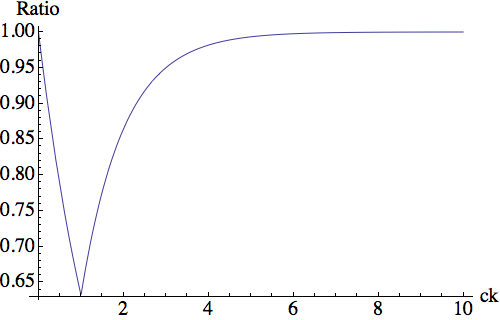
\includegraphics[width=5cm]{images/Sri_Original.png}
\caption{Approximation Ratio as a function of $ck$ }\label{fig:simple_approx}
\end{figure}

%Now suppose that $G$ is generated and $H$ is sampled using the same
%processes as described above. The next theorem, extends the above
%bounds to the $(c,a)$-graph recommendation problem where $a>1$.
%In particular if we set $a=1$, we will obtained the estimate from the original analysis.

%Now, we can perform a similar analysis as before. In
%particular, 
For the general $(c, a)$-recommendation subgraph problem, if $ck>a$, then the problem is easy on average. This
is in comparison to the trivial estimate of $cl$. For a fixed $a$, a
random solution gets better as $ck$ increases because the decrease in
$e^{-ck}$ more than compensates for the polynomial in $ck$ next to
it. However, in the more realistic case $ck<a$, we need to use the
trivial estimate of $ckr/a$, and the analysis for $a=1$ does not extend here. 
The following table shows how large 
$ck$ needs to be for the solution to be 95\% optimal for different
values of $a$.\vs

%In both this analysis and the previous one, $ck$ is the average degree
%of a vertex $v\in R$ in our chosen subgraph. The original analysis
%showed that if $ck>1$, then the sampling algorithm will probably cover
%every vertex in $R$ since the expected degree of each vertex is large.
%On the other hand if $ck$ is small ($ck < 1$) then the best possible
%solution is obtained when none of the vertices in $R$ has degree
%greater than 1. \vs

%If $ck<1$, then we do not cover very
%many vertices in $R$, but we also do not cover many vertices more than
%once. Since the optimal solution in this case was correspondingly low,
%our solution was good in the $a=1$ case. However, when $a<1$, the fact
%that our edges are well-dispersed only hurts our solution because we
%need to concentrate the edges on specific nodes in $R$ that will
%eventually count in the objective. 

\begin{figure}[h]
  \centering
  \begin{tabular}{ |c|c|c|c|c|c| }
    \hline
    $a$ & 1 & 2 & 3 & 4 & 5 \\ \hline
    $ck$ & 3.00 & 4.74 & 7.05 & 10.01 & 13.48 \\
    \hline
  \end{tabular}
  \caption{The required $ck$ to obtain 95\% optimality for $(c, a)$-recommendation subgraph}
\end{figure} 

We close out this section by showing that the main result that holds in expectation also hold with high probability. 
While Chernoff bounds are usually stated for independent variables, the
variant below holds for any number of pairwise non-positively correlated
variables.

\begin{thm}\label{negative_corr_chernoff}~\cite{AugerDoerr2011}
Let $X_1,\ldots, X_n$ be non-positively correlated variables. If $X=\sum_{i=1}^n X_i$, then for any $\delta\geq 0$
\[ Pr[X \geq (1+\delta)\E[X] ] \leq \left(\frac{e^\delta}{(1+\delta)^{1+\delta}}\right)^{\E[X]} \]
\end{thm}

Using this we can convert our expectation result to one that holds 
with high probability.

\begin{thm}
Let $S$ be the random variable denoting the number of vertices $v \in R$ such that $\deg_{H}(v)\geq 1$. Then
$ S \leq r(1-2\exp(-ck))$ with probability at most $(e/4)^{r(1-\exp(-ck))}$.
\end{thm}

\begin{proof}
We can write $S$ as $\sum_{v\in R} 1-X_v$ where $X_v$ is the indicator
variable that denotes that $X_v$ is matched. Note that the variables
$1-X_v$ for each $v\in R$ are non-positively correlated. In
particular, if $N(v)$ and $N(v')$ are disjoint, then $1-X_v$ and
$1-X_{v'}$ are independent. Otherwise, $v$ not claiming any edges can
only increase the probability that $v'$ has an edge from any vertex
$u\in N(v)\cap N(v')$. Also note that the expected size of $S$ is
$r(1-\exp(-ck))$ by Theorem \ref{original_result}. Therefore, we can
apply Theorem \ref{negative_corr_chernoff} with $\delta=1$ and obtain
the result.
\end{proof}

\subsection{The Greedy Algorithm}
\label{greedy}
The results in the previous section concentrated on producing nearly
optimal solutions in expectation. In this section, we will show that
it is possible to obtain good solutions regardless of the model that
generated the recommendation subgraph. \vs

We analyze the following
natural greedy algorithm. Consider each vertex in $R$ that has not been selected
into $H$ in some arbitrary order. If there is some $v \in R$ that has $a$ neighbors
in $L$ all of which have degree less than $c$, add $v$ and these edges to $H$ breaking
ties arbitrarily.

\begin{thm}
The greedy algorithm achieves $1/(a+1)$-approximation ratio for the $(c,a)$-graph
recommendation problem.
\end{thm}
\begin{proof}
Let $R_{GREEDY}, R_{OPT}\subseteq R$ be the set of vertices that have
degree $\geq a$ in the greedy and optimal solutions respectively. Note
that any $v \in R_{OPT}$ along with neighbors $\{u_1,\ldots u_a\}$
forms a set of candidate edges that can be used by the greedy
algorithm. So we can consider $R_{OPT}$ as a candidate pool for
$R_{GREEDY}$. Each selection that the greedy algorithm makes might result in
some of the candidates becoming infeasible. But as long as the candidate pool
is not depleted, the greedy algorithm can continue. 
Each time the greedy algorithm selects some vertex $v\in
R$ with edges to $\{u_1,\ldots, u_a\}$, we remove $v$ from the candidate pool. 
If any $u_i$ had degree $c$ in the optimal solution, we would also need to
remove an arbitrary vertex $v_i\in R$ adjacent to $u_i$ from the optimal
solution. In other words, by using an edge of $u_i$, we force it to
not use an edge it used to some other $v_i$, which might cause the
degree of $v_i$ to go below $a$. Therefore, at each step of
the greedy algorithm, we have to remove at most $a+1$ vertices from
the candidate pool. Since our candidate pool has size $OPT$, the
greedy algorithm can not stop before it has added $OPT/(a+1)$
vertices to the solution.
\end{proof}

\begin{figure}[h]
\centering
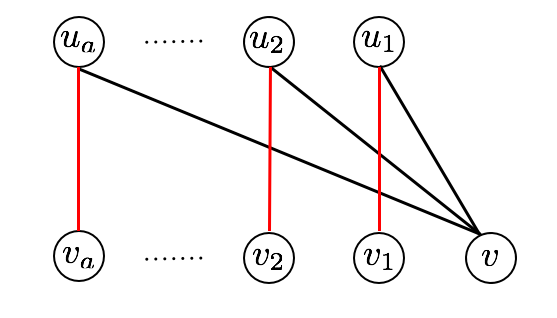
\includegraphics[width=.5\textwidth]{images/greedy.png}
\begin{minipage}[h]{.8\linewidth}
\caption{This diagram shows one step of the greedy algorithm. When $v$ selects edges to $u_1,\ldots, u_a$, it potentially removes $v_1,\ldots, v_a$ from the pool of candidates that are avaiable. The potentially invalidated edges are shown in red.}
\end{minipage}
\end{figure}

Note that this approximation guarantee is as good as we can expect.
If we set $a=1$ then we obtain the familiar
$1/2$-approximation of the greedy algorithm for matchings. 
As in matchings, randomizing the order in
which the vertices are processed still leaves a constant factor gap
in the size of the solution\cite{KarpVaziraniVazirani1990}.
Despite this result, the greedy algorithm fares much better when we
give it the same expectation treatment we have given the sampling
algorithm. We now prove the near optimality of the greedy algorithm for the
$(c, a)$-recommendation subgraph problem.

\begin{thm}
Let $G=(L,R,E)$ be a graph drawn from the $G_{l,r,p}$. If $S$ is the size of the $(c,a)$-recommendation subgraph produced by the greedy algorithm, then:
\[ \E[S] \geq r - \frac{a(lp)^{a-1}}{p}\]
\end{thm}
\begin{proof}
Note that if edges are generated uniformly, we can consider the
graph as being revealed to us one vertex at a time as the greedy
algorithm runs. In particular, consider the event $X_i$ that the
greedy algorithm matches the $(i+1)^{th}$ vertex it inspects. While,
$X_{i+1}$ is dependent on $X_1,\ldots, X_i$, the worst condition for
$X_{i+1}$ is when all the previous $i$ vertices were from the same
vertices in $L$, which are now not available for matching the
$(i+1)^{th}$ vertex. The maximum number of such invalidated vertices
is at most $\lceil i/c \rceil$. Therefore, the probability that fewer
than $a$ of the at least $l-\lceil i/c \rceil $ available 
vertices have an edge to this vertex is at most $\Pr[Y\sim Bin(l-\frac{i}{c},p): Y < a]$.
Using the approximation that
\[ \Pr[Y\sim Bin(l-\frac{ia}{c},p): Y < a] \leq a(1-p)^{l-\frac{ia}{c}-a+1}(lp)^{a-1}\]
and summing over all the $X_i$ using the linearity of expectation,
we obtain
\begin{align*}
      \E[S]
&\geq r - \sum_{i=0}^{r-1} \E[\lnot X_i] \\
&\geq r - \sum_{i=0}^{r-1} \Pr[Y \sim Bin(l-\frac{ia}{c},p): Y < a] \\
&\geq r - \sum_{i=0}^{r-1}a(1-p)^{l-\frac{ia}{c}-a+1}[lp-\frac{iap}{c}]^{r-1} \\
&\geq r - a(lp)^{r-1}\sum_{i=0}^{r-1}(1-p)^{l-\frac{ia}{c}-a+1} \geq r - \frac{a(lp)^{a-1}}{p}\\
\end{align*}
\end{proof} 

\subsection{Existence of Perfect Recommendation Subgraphs}
Define a \emph{perfect} $(c,a)$-recommendation subgraph on $G$ to be a subgraph $H$ such that
$deg_H(u)\leq c$ for all $u\in L$ and $deg_H(v)=a$ for
$\min(r,cl/a)$ of the vertices in $R$. In this section we will
prove a sufficient condition for perfect $(c,a)$-recommendation
subgraphs to exist in a bipartite graph $G$ under the Erd\"os-Renyi model\cite{ErdosRenyi59} where edges are sampled
uniformly and independently with probability $p$. 
We use the algorithm we propose to prove this condition as a candidate to compare against random choice and greedy in our tests.
Our result relies on
the following characterization of perfect matchings.

\begin{thm}\cite{Janson2011}
\label{random_matching_threshold}
Let $G$ be a bipartite graph drawn from $G_{n, n, p}$. If $p \geq \frac{\log n -
\log\log n}{n}$, then as $\lim_{n\to\infty}$ probability that G has a perfect
    matching approaches 1.
\end{thm}

We will prove that a perfect $(c,a)$-recommendation subgraph exists in
random graphs with high probability by building it up from $a$
matchings each of which must exist with high probability if $p$ is
sufficiently high. In particular, we show that $p$ only needs to
be $\Omega(\frac{\log n}{n})$ for this to succeed. 
%While the theorem is stated for
%the case when $a \leq c$, it applies equally well to the $a > c$
%case by partitioning $L$ instead of $R$ in the following proof.

\begin{thm}
Let $G$ be a random graph drawn from $G_{l, r, p}$ with $p\geq a\frac{\log l-\log\log
l}{l}$ and $kc \geq a$, then the probability that $G$ has a perfect $(c, a)$-recommendation
subgraph tends to 1 as $l,r\to\infty$.
\end{thm}

\begin{proof}
Given the size and the degree constraints of $L$, at most $lc/a$
vertices in $R$ can have degree $a$ in a $(c,a)$-recommendation subgraph. We
therefore restrict $R$ to an arbitrary subset $R'$ of size $lc/a$.
Next, we pick an enumeration of the vertices in $R'=\{v_0,\ldots, v_{lc/a-1}\}$
and add these vertices into $a$ subsets by defining
$R_i = \{v_{(i-1)l/a}, \ldots, v_{(i-1)l/a+l-1}\}$ for each $1\leq i\leq c$ where
the arithmetic in the indices is done modulo $lc/a$. Note both $L$ and all of
the $R_i$'s have size $l$. \vs

Using these new sets we define the graphs $G_i$ on the bipartitions
$(L, R_i)$. Since the sets $R_i$ are intersecting, we cannot define the
graphs $G_i$ to be induced subgraphs. However, note that each vertex $v\in R'$
falls into exactly $a$ of these subsets. Therefore, we can uniformly randomly assign each
edge in $G$ to one of $a$ graphs among $\{G_1,\ldots, G_c\}$ it can fall into,
and make each of those graphs a random graph. In fact, while the different
$G_i$ are coupled, taken in isolation we can consider any single $G_i$ to be
drawn from the distribution $G_{l,l,p/a}$ since $G$ was drawn from $G_{l,r,p}$.
Since $p/a \geq (\log l - \log\log l)/l$ by assumption, we conclude by
Theorem~\ref{random_matching_threshold}, the probability that a particular
$G_i$ has no perfect matching is $o(1)$. \vs

Considering $c$ to be fixed, by a union bound, we then conclude that except
for a $o(1)$ probability, each one of the $G_i$'s has a perfect matching. By
superimposing all of these perfect matchings, we can see that every vertex in
$R'$ has degree $a$. Since each vertex in $L$ is in exactly $c$ matchings, each
vertex in $L$ has degree $c$. It follows that except for a $o(1)$ probability
there exists a $(c,a)$-recommendation subgraph in $G$.
\end{proof}

\subsection{Approximation Algorithm Using Perfect Matchings}

The above result now enables us to design a near linear time
algorithm with a $(1-\epsilon)$ approximation guarantee
to the $(c,a)$-recommendation subgraph problem by leveraging
combinatorial properties of matchings.

\begin{thm}
Let $G$ be drawn from $G_{l,r,p}$ where $p \geq a\frac{\log l - \log\log l}{l}$. Then there
exists an algorithm that can find a $(1-\epsilon)$-approximation in time
$O(\frac{|E|c^2}{\epsilon})$ with probability $1-o(1)$.
\end{thm}
\begin{proof}
As with the proof of the previous theorem, we can arbitrarily restrict $R$ to a
subset of size $lc/a$ and divide $R$ into sets $R_1,\ldots,R_c$ such that each
vertex in $R$ is contained in exactly $a$ of the sets. Using the previous
theorem, we know that each of the graphs $G_i$ has a perfect matching with high
probability. These perfect matchings can be approximated to a $1-\epsilon/c$
factor by finding matchings that do not have augmenting paths of length
$\geq 2c/\epsilon$~\cite{LovaszPlummer1983}. This can be done for each
$G_i$ in $O(|E|c/\epsilon)$ time. Furthermore, the union of unmatched vertices
makes up an at most $c(\epsilon/c)$ fraction of $R'$.
\end{proof}


\section{Computational Results}

We simulated performance of our algorithms on random graphs generated
by the graph models we outlined. In the following graphs each data
point is obtained by averaging the measurements over 10 random
graphs. Figures~\ref{fig:a=1:1} and \ref{fig:a=1:2} show that the
lower bound we calculated for the expected performance of the sampling
algorithm accurately captures the behavior of the sampling algorithm
when $a=1$. Indeed, the inequality we used is an accurate
approximation of the expectation, up to lower order terms. The random
sampling algorithm does well, both when $c$ is low and high, but
falters when $ck=1$. The greedy algorithm performs better than the
random sampling algorithm in all cases, but its advantage vanishes as
$c$ gets larger. Note that the dip in the graphs when $cl=ar$, at
$c=4$ in Figure~\ref{fig:a=1:1} and $c=2$ in Figure~\ref{fig:a=1:2} is
expected and was previously demonstrated in Figure 1.  In all the
plots below, the red, blue and yellow lines denote the approximation
ratio of the greedy, sampling and partitioning algorithms respectively
wrt the upper-bounds of the optimal that we described before.

\begin{figure}[h]
\centering
\begin{minipage}[h]{0.45\textwidth}
\centering
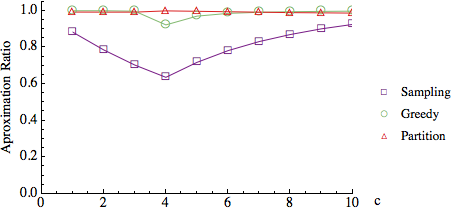
\includegraphics[width=0.8\textwidth]{images/l=25000,r=100000_Greedy_vs_Naive.png}
\caption{Approximation ratios when $|L|=25$k, $|R|=100$k, $d=20$, $a=1$}\label{fig:a=1:1}
\end{minipage}
\hspace{0.2cm}
\begin{minipage}[h]{0.45\textwidth}
\centering
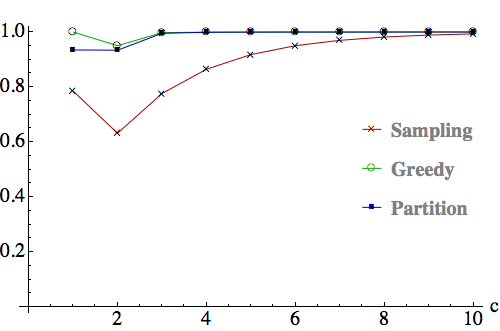
\includegraphics[width=0.8\textwidth]{images/l=50000,r=100000_Greedy_vs_Naive.png}
\caption{Approximation ratios when $|L|=50$k, $|R|=100$k, $d=20$, $a=1$}\label{fig:a=1:2}
\end{minipage}
\end{figure}


% Can we show the graph for larger c? Maybe up to 20?
% Also I can't believe that greedy is optimal. I am still tempted to say that
% greedy will do badly when d is small. Like d < 5.

In contrast to the case when $a=1$, the sampling algorithm performs
worse when $a>1$ but performs increasingly better with $c$ as
demonstrated by Figures~\ref{fig:a=2} and \ref{fig:a=4}. The greedy
algorithm continues to produce solutions that are nearly optimal,
regardless of the settings of $c$ and $a$. Therefore, our simulations
suggest that in many cases a software engineer can simply design the
sampling method for solving the $(c, a)$-recommendation subgraph
problem. In those cases where the sampling is not suitable we still
find that the greedy does adequately given its simplicity in
implementation.

\begin{figure}[h]
\centering
\begin{minipage}[h]{0.45\textwidth}
\centering
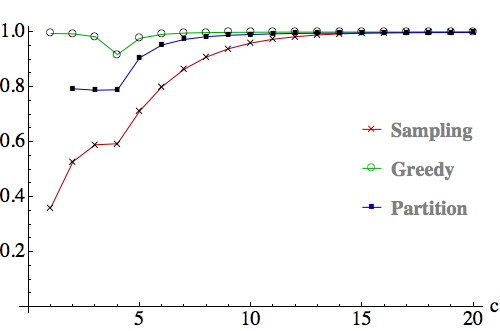
\includegraphics[width=0.8\textwidth]{images/l=50000,r=100000,a=2_Greedy_vs_Naive.png}
\caption{Approximation ratios when $|L|=50$k, $|R|=100$k, $d=20$, $a=2$}\label{fig:a=2}
\end{minipage}
\hspace{0.2cm}
\begin{minipage}[h]{0.45\textwidth}
\centering
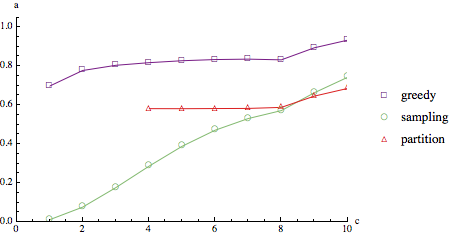
\includegraphics[width=0.8\textwidth]{images/l=50000,r=100000,a=4_Greedy_vs_Naive.png}
\caption{Approximation ratios when $|L|=50$k, $|R|=100$k, $d=20$, $a=4$}\label{fig:a=4}
\end{minipage}
\end{figure}

\section{Realistic Models of Recommendation Graphs}
%We realize that the models described previously are a bit
%theoretical.
Even though we studies the fixed-degree model in detail, recommendation systems based on relevance in practice
will not have edges that are spread uniformly at random. Items that are
about specific topics are much more likely to interlink within
themselves than to those outside that topic, leading to
clusters of recommendations.

To understand this substructure in underlying
graphs in practice, we compiled results from several e-commerce retailers that
have been aggregated and anonymized in the table shown below. For each
retailer, we compiled the product ontology present within the
site that places a product in this tree-like categorization. E.g., a
juicer called ``Breville Juice Fountain Plus'' is in the tree path:
Home $\rightarrow$ Juicers $\rightarrow$ High Speed Juicers
$\rightarrow$ Breville Juice Fountain Plus. We then examined the
recommendations from products at different depths of the hierarchy. In
the table in Figure~\ref{fig:hier} we examined the edges adjacent to
products at depth 4 or greater. We calculated the percentage of edges
connecting to products that had different least common ancestors (LCA) with the current product.  We
then randomized the edges so that we can compare how the graph would
have looked if there was no substructure and re-calculate the
distribution of the edges and the LCA levels. We noticed that the
uniform distribution had edges that had very shallow LCA indicating that
most edges did not follow the product hierarchy while in reality,
the endpoints of edges recommended had much deeper LCA meaning recommendation edges were clustered based on the product hierarchy. This led us
to formalize this new model of input graphs that we study in Subsection~\ref{hierarchy}
as the {\em hierarchical tree model}.

\begin{figure}[h]
  \centering
  \begin{tabular}{ |c|c|c|c|c|c|c|c|c|c| }
    \hline
    $LCA Level$ & 0 & 1 & 2 & 3 & 4 & 5 & 6 & 7 \\ \hline
    Uniform & 13.4 & 69.7 & 12.5 & 2.6 & 1.2 & 0.6 & 0.0 & 0.0 \\ \hline
    Hierarchical & 7.1 & 1.9 & 8.0 & 24.9 & 52.3 & 5.5 & 0.2 & 0.1\\
    \hline
  \end{tabular}
  \caption{Percent edges for depth-4 products by LCA of endpoints in reality (Hier) and simulated Uniform.}\label{fig:hier}
\end{figure}

In a second analysis, we simply truncated the product hierarchy
at depth 3 and collected the resulting disjoint clusters in the hierarchy. We
then examined all the recommendations and partitioned them into those going between each pair of these clusters. In a uniform distribution, we would expect the
edges to be equally likely to span across each pair of clusters
(assuming clusters are equal sized). But what we observed was that
different pairs of clusters had different edge-densities. For instance, an Espresso Machine might point more to other Coffee Machines or
Coffee Beans (note that Coffee Beans and Espresso Machine might share
no LCA apart from the root) than to other clusters. These results are
shown in Figure~\ref{fig:cart-emp} that clearly demonstrates that these
clusters exist and have different densities than the uniform sampling model. This
motivated us to define and study the {\em cartesian product model} in
Subsection~\ref{cartesian} which is orthogonal to the uniform and
hierarchical tree models. Finally, in Section~\ref{weighted}, we study the {\em weighted model}
which assigns weights to the graph edges so that we can incorporate strengths and traffic
patterns across a website besides just relevance-based recommendations.

\begin{figure}
\centering
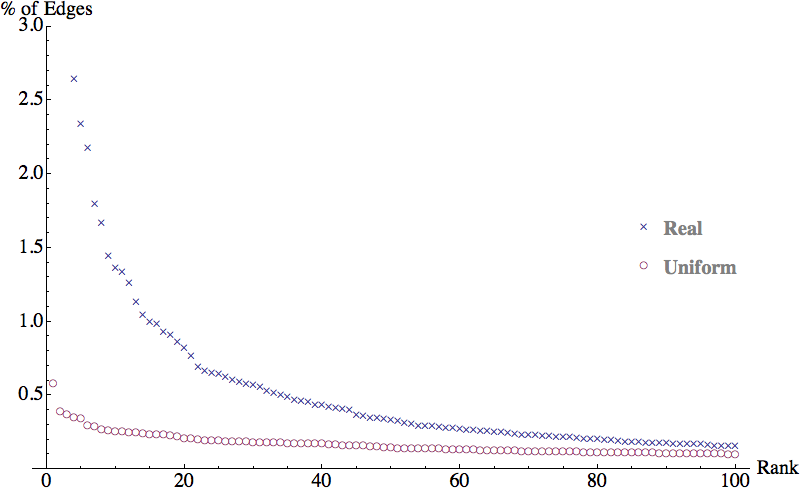
\includegraphics[width=0.5\textwidth]{images/cartesian_histogram.png}
\begin{minipage}{1\textwidth}
\caption{Histogram of percent edges between pairs of clusters. The long tail is omitted.}
\label{fig:cart-emp}
\vspace{-0.2in}
\end{minipage}
\end{figure}

\subsection{Hierarchical Tree Model}
\label{hierarchy}

%We assume that we are given a bipartite graph $G=(L,R,E)$. 
In this model, the vertex sets $L$
and $R$ are the leaf sets of two full binary trees $T_L$ and $T_R$ of
depth $D$ where there is a one-to-one correspondence between the
subtrees of these two trees. We also assume that each branching in
both $T_L$ and $T_R$ splits the nodes evenly into the two
subtrees. As in the previous sections, we set $|L|/|R|=k$,
and require that this ratio is still $k$ if we divide the size of any subtree on the left
and that of its corresponding subtree on the right. For simplicity of notation, we
will use a subtree and its leaf set interchangeably. We assume that the trees are
fixed in advance but the bipartite recommendation graph $G = (L, R, E)$ is generated probabilistically according to
the following procedure. Let $u\in L$ and $T_L^0, \ldots T^{D-1}_L$ be
the subtrees it belongs at depths $0,\ldots, D-1$. Also, let
$T_R^0,\ldots, T_R^{D-1}$ be the subtrees on the right that correspond
to these trees on the left. We let $u$ make a recommending edge to $d_{D-1}$ of
the vertices in $T_{R}^{D-1}$, $d_{D-2}$ edges to the vertices in
$T_{R}^{D-2} \backslash T_{R}^{D-1}$ and so on. The $d_i$ edges out of $u$ are chosen uniformly from $T_R^i \setminus T_R^{i+1}$.
Let $d = d_{0} + \ldots + d_{D-1}$.\vs

\begin{figure}[b]
\vspace{-0.2in}
\centering
\begin{minipage}{0.45\textwidth}
\centering
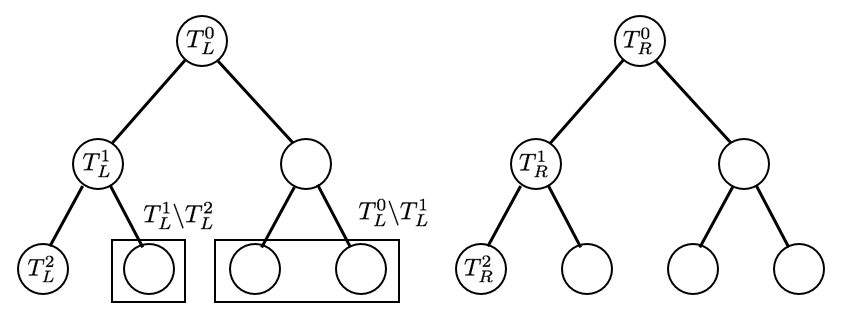
\includegraphics[width=1.1\textwidth]{images/hierarchy_tree.png}
%\begin{minipage}[h]{0.7\textwidth}
\caption{This diagram shows the notation we use for this model and the 1-to-1 correspondence of subtrees.}\label{fig:hierarchy}
\end{minipage}
\hspace{0cm}
\begin{minipage}{0.45\textwidth}
\centering
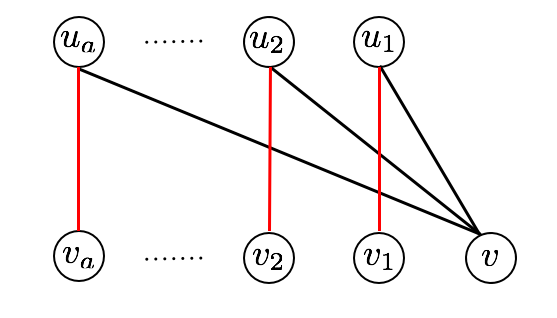
\includegraphics[width=0.9\textwidth]{images/greedy.png}

%\begin{minipage}[h]{.8\linewidth}

\vspace{-0.3in}
\caption{When $v$ selects edges to $u_1,\ldots, u_a$, it can remove $v_1,\ldots, v_a$ from candidates. Potentially invalidated edges shown in red.}

%\end{minipage}
\label{fig:greedy}
\end{minipage}
\end{figure}




Our goal now is to find a variant of matching~\cite{Gabow1983} in this
graph that is close to optimal in expectation for the case of $a=1$. That is, our degree
upper and lower bounds on vertices in $L$ and $R$ are $c$ and 1
respectively. Let $c = c_0 + \ldots + c_{D-1}$ be similar to how we
defined $d$.  To combine the analysis of the randomness of the
algorithm and the randomness of the graph, the algorithm will pick
$c_{i}$ edges uniformly from among the $d_{i}$ edges going to each
level of the subtree. This enables us to think of the subgraph our
algorithm finds as being generated by the identical graph generation
process, but with fewer neighbors selected. With this model and
parameters in place, we can have the following analog of our main
theorem for $a=1$ for the hierarchical model and is proved in Appendix~\ref{sec:appendix}.

\begin{thm}
Let $S$ be the subset of edges $v\in R$ such that $\deg_H(v) \geq 1$ in the hierarchical tree model. Then
\[ \E[S] \geq r(1-\exp(-ck)) \]
\end{thm}

%\begin{proof}
%Let $v\in R$ and let $T_L^{D-1}, T_L^{D-2}\backslash T_L^{D-1},
%\ldots, T_L^0\backslash T_L^1$ be the sets it can take edges
%from. Since $T_L$ and $T_R$ split perfectly evenly at each node the
%vertices in these sets will be chosen from $r_{D-1}, r_{D-1},
%r_{D-2},\ldots, r_{1}$ vertices in $R$ as neighbors,
%where $r_i$ is the size of subtree of the right tree rooted at depth
%$i$. Furthermore, each of these sets described above have size
%$l_{D-1}, l_{D-1}, l_{D-2}, \ldots, l_{1}$ respectively, where $l_i$
%is the size of a subtree of $T_L$ rooted at depth $i$. It follows that
%the probability that $v$ does not receive any edges at all is at most
%
%\begin{align*}
%	      \Pr[\lnot X_v]
%	&=    \left(1-\frac{1}{r_{D-1}}\right)^{c_0l_{D-1}}\prod_{i=1}^{D-1}\left(1 - \frac{1}{r_i}\right)^{c_{D-i} l_i} \\
%	&\leq \exp\left(-\frac{l_{D-1}}{r_{D-1}}c_0\right)\prod_{i=1}^{D-1} \exp\left(-\frac{l_i}{r_i}c_{D-i}\right) \\
%	&=    \exp\left(-(c_0 + \ldots + c_{D-1})k\right) \\
%	&=    \exp(-ck)
%\end{align*}
%
%Since this is an indicator variable, it follows that
%\[ \E[S] = \E\left[\sum_{v \in R} X_v \right] \geq r \left(1-\exp(-ck)\right) \]
%\end{proof}

Note that this is the same result as we obtained for the fixed degree
model in Section \ref{fixed-degree}. In fact, the approximation
guarantees when $ck \ll 1$ or $ck \gg 1$ hold exactly as before.\vs

The algorithmic sampling of $H$ is convenient in this model because we separated
out the edge generation process at a given depth from the edge
generation process at deeper subtrees. 
%There is no ambiguity as to why
%an edge is in the underlying graph. That is, 
If we superimpose $T_L$
and $T_R$, then an edge between $u_l\in L$ and $v_r\in R$ must have
come from an edge generated by the process corresponding to the lowest common ancestor of $u_l$ and $v_r$ in the same hierarchy. This way, the algorithm can actually sample intelligently and in the same way that the graph was generated in the first place, which is also the key to our simple analysis. Note
that we do not have to assume that the trees $T_L$ and $T_R$ are
binary. We only need the trees to be regular and evenly divided at
each vertex since the proof only relies on the proportions of the
sizes of the subtrees in $T_L$ and $T_R$.


\subsection{Cartesian Product Model}
\label{cartesian}
We can see another shortcoming of the uniform graph model if we think
of products as being clustered into categories. This is similar to the
hierarchical tree mode, but our assumptions are weaker in that we don't
mandate a complete hierarchy and that the clusters can be unrelated. In
such a model, we would expect many more recommendation edges to be
intra-cluster edges rather than inter-cluster edges.


This finding motivates the cartesian product model where we assume that
$L$ has been partitioned into $t$ subsets $L_1,\ldots, L_t$ and
that $R$ has been partitioned into $t'$ subsets $R_1,\ldots,
R_{t'}$, and we assign different densities to different terms in their cartesian product. For convenience, we let $|L_i| = l_i$ and $|R_i|=r_i$. Given
this, for each $1\leq i\leq t$ and each $1\leq j\leq t'$,
we let $G[L_i, R_j]$ be an instance of the fixed degree model with
$d=d_{ij}$. However, we require that for all $i$, we have $\sum_{j=1}^{t'}
d_{ij} = d$ for some fixed $d$. Also we require that we have fixed in
advance $c_{ij} \leq d_{ij}$ for each $1\leq i\leq t$ and $1\leq j\leq t'$ that
satisfy $\sum_{j=1}^{t'} c_{ij} = c$ for all $i$ for some fixed $c$.
To sample $H$ from $G$, we sample $c_{ij}$ neighbors for each
$u_i\in L_i$ from $R_i$. Letting $S$ be the set of vertices in
$v\in R$ that satisfy $\deg_H(v)\geq 1$, we can show the following theorem
that is proved in Appendix~\ref{sec:appendix}.

\begin{thm}
Let $S$ be the subset of edges $v\in R$ such that $\deg_H(v) \geq 1$ in the cartesian product model. Then
%\vspace{-0.1in}
\[ \E[S] \geq r - \sum_{j=1}^{t'} r_j \exp\left(-\sum_{i=1}^t c_{ij} \frac{l_i}{r_j}\right)\]
\end{thm}
%\begin{proof}
%Let $v_j \in R_j$ be an arbitrary vertex and let $X_{v_j}$ be the
%indicator variable for the event that $\deg_H(v_i) \geq 1$. The
%probability that none of the neighbors of some $u_i\in R_i$ is $v_j$
%is exactly $(1-\frac{1}{r_j})^{c_{ij}}$. It follows that the
%probability that the degree of $v_j$ in the subgraph $H[L_i,R_j]$ is 0
%is at most $(1-\frac{1}{r_j})^{c_{ij}l_i}$. Considering this
%probability over all $R_j$ gives us:
%\[ \Pr[X_{v_i} = 0] = \prod_{i=1}^{t} \left(1-\frac{1}{r_j}\right)^{c_{ij} l_i} \leq \exp\left(-\sum_{i=1}^t c_{ij} \frac{l_i}{r_j}\right)\]
%
%By linearity of expectation $\E[S] = \sum_{i=1}^{t'} r_i \E[X_{v_i}]$,
%so it follows that
%\[ \E[S] \geq \sum_{j=1}^{t'} r_j \left(1-\exp\left(-\sum_{i=1}^t c_{ij} \frac{l_i}{r_j}\right)\right) = r - \sum_{j=1}^{t'} r_j \exp\left(-\sum_{i=1}^t c_{ij} \frac{l_i}{r_j}\right)\]
%\end{proof}

%This model is interesting because it can capture a broader set of
%recommendation subgraphs than the fixed degree model. However, it is
%difficult to estimate how good a solution will be without knowing
%the sizes of the sets in the partitions. We note that we
%obtain the approximation guarantee of $(1-\exp(-ck))$ provided that
%$l_i/r_j = k$ for all $i$ and $j$ where $k$ is some fixed
%constant.
An interesting point about this model and the algorithm
we described for sampling $H$ is that we are free to select $c_{ij}$.
In particular, $c_{ij}$ can be chosen to maximize the
approximation guarantee in expectation we obtained above using
gradient descent or other first order methods prior to running the
recommendation algorithm to increases the quality of the solution.

\subsection{Weighted Model}
\label{weighted}
The fixed degree model of Section \ref{fixed-degree} is a simple and
convenient model, but the assumption that all recommendations hold the
same weight is unrealistic. This motivates fixing the graph to be the
complete bipartite graph $K_{l,r}$, and giving the edges i.i.d weights
with mean $\mu$. We modify the objective function accordingly, so that
we count only the vertices in $R$ which have weight $\geq 1$. If we
assume that $ck\mu \geq 1+\epsilon$ for some $\epsilon > 0$, then
the naive sampling solution we outlined in Section \ref{fixed-degree}
still performs exceptionally well. If we let $S$ be the size of the
solution produced by this algorithm. We have the following theorem that is
proved in Appendix~\ref{sec:appendix}.

\begin{thm}
Let $G=K_{l,r}$ be a complete bipartite graph where the edges have i.i.d. weights and come from a distribution with mean $\mu$ that is supported on $[0,b]$; Assume that $ck\mu \geq 1+\epsilon$ for some $\epsilon > 0$. If the algorithm from Section \ref{fixed-degree} is used to sample a subgraph $H$ from $G$, then
\[ \E[S] = \sum_{v\in R} \E[X_v] = r\left(1-\exp\left(-\frac{2l\epsilon^2}{b^2}\right)\right) \]
\end{thm}

There are two things to note about this variant. The first is that
since the variables $X_v$ are negatively correlated, our results in
Subsection \ref{fixed-degree} can be extended to the results of this
section. The second is that the condition that $W_{uv}$ are i.i.d
is not necessary to obtain the full effect of the analysis. Indeed,
the only place in the proof where the fact that $W_{uv}$ are i.i.d
is when we argued that $X_{uv}$ is large with high probability by a
Hoeffding bound. For the bound to apply, it is sufficient to assume
that $W_{uv}$ for all $v$ are independent. In particular, it is
possible that $W_{uv}$ for all $u$ are inter-dependent. This allows
us to assume a weight distribution that depends on the strength of
the recommender and the relevance of the recommendation separately.

\section{Conclusions}

In this paper we proposed several different models for explaining how
recommendation subgraphs arise probabilistically and how optimization
problems on these graphs can be solved, but there is much more that
can be done both on the theoretical and the empirical fronts. On the
theory side the biggest open problem is the hardness of the general
$(c, a)$-recommendation subgraph problem. For specific values of $c$
and $a$ we know polynomial time algorithms. For e.g., $a=1$ leads to
either bipartite matching or fractional matching which can be solved
in polynomial time but the hardness of the general problem remains
open. On the empiral side, the graph models that we introduced can be
made richer. For example, the hierarchical graphs require the trees to
be balanced and of the same size which is constraining. The edge
weights on the weighted graph is sampled from a distribution as
opposed to being arbitrary. We expect the research community and our
future work to follow-up along both directions in the future.


%\begin{enumerate}

%\item We do not know of a polynomial time algorithm that can solve the
%  $(c, a)$-recommendation subgraph problem. For specific values of $c, a$ we
%  know polynomial time algorithms. For e.g., $a=1$ leads to either
%  bipartite matching or fractional matching which can be solved in
%  polynomial time. 

%\item In practice, there might exist several different
%  recommendation subgraphs based on different features. For example,
%  two people might be related because they went to the same 
%  school, or because they live in the same city, or because they
%  would complete a large number of triangles, etc. It's worthwhile
%  to investigate how such graphs can be combined into one, or how
%  an optimization problem can be solved using all such 
%  recommendation subgraphs simultaneously.

%\item We should devise metrics that can evaluate how well a
%  recommendation subgraph fits a given model and conduct some parameter
%  fitting experiments to see how well actual recommendation subgraphs
%  which arise in practice fit our models.

%\item We should implement the sampling and the greedy algorithms
%  given in the paper to see if they can solve to near optimality
%  the graph recommendation problems that arise in practice.

%\end{enumerate}


\pagebreak
\setcounter{page}{1}
\bibliography{cite}{}
\bibliographystyle{plain}

\pagebreak
\appendix
\section{Proofs of More General Models}

\begin{thm}
Let $S$ be the subset of edges $v\in R$ such that $\deg_H(v) \geq 1$. Then
\[ \E[S] \geq r(1-\exp(-ck)) \]
where the expectation is over $G$ and $H$.
\end{thm}

\begin{proof}
Let $v\in R$ and let $T_L^{D-1}, T_L^{D-2}\backslash T_L^{D-1},
\ldots, T_L^0\backslash T_L^1$ be the sets it can take edges
from. Since $T_L$ and $T_R$ split perfectly evenly at each node the
vertices in these sets will be chosen from $r_{D-1}, r_{D-1},
r_{D-2},\ldots, r_{1}$ vertices in $R$ as neighbors,
where $r_i$ is the size of subtree of the right tree rooted at depth
$i$. Furthermore, each of these sets described above have size
$l_{D-1}, l_{D-1}, l_{D-2}, \ldots, l_{1}$ respectively, where $l_i$
is the size of a subtree of $T_L$ rooted at depth $i$. It follows that
the probability that $v$ does not receive any edges at all is at most

\begin{align*}
	      \Pr[\lnot X_v] 
	&=    \left(1-\frac{1}{r_{D-1}}\right)^{c_0l_{D-1}}\prod_{i=1}^{D-1}\left(1 - \frac{1}{r_i}\right)^{c_{D-i} l_i} \\
	&\leq \exp\left(-\frac{l_{D-1}}{r_{D-1}}c_0\right)\prod_{i=1}^{D-1} \exp\left(-\frac{l_i}{r_i}c_{D-i}\right) \\
	&=    \exp\left(-(c_0 + \ldots + c_{D-1})k\right) \\
	&=    \exp(-ck)
\end{align*}

Since this is an indicator variable, it follows that 
\[ \E[S] = \E\left[\sum_{v \in R} X_v \right] \geq r \left(1-\exp(-ck)\right) \]
\end{proof}

\begin{thm}
With $S$, $G$ and $H$ defined as above, we have
\[ \E[S] \geq r - \sum_{j=1}^{t'} r_j \exp\left(-\sum_{i=1}^t c_{ij} \frac{l_i}{r_j}\right)\]
where the expectation is over $G$ and $H$.
\end{thm}
\begin{proof}
Let $v_j \in R_j$ be an arbitrary vertex and let $X_{v_j}$ be the
indicator variable for the event that $\deg_H(v_i) \geq 1$. The
probability that none of the neighbors of some $u_i\in R_i$ is $v_j$
is exactly $(1-\frac{1}{r_j})^{c_{ij}}$. It follows that the
probability that the degree of $v_j$ in the subgraph $H[L_i,R_j]$ is 0
is at most $(1-\frac{1}{r_j})^{c_{ij}l_i}$. Considering this
probability over all $R_j$ gives us:
\[ \Pr[X_{v_i} = 0] = \prod_{i=1}^{t} \left(1-\frac{1}{r_j}\right)^{c_{ij} l_i} \leq \exp\left(-\sum_{i=1}^t c_{ij} \frac{l_i}{r_j}\right)\]

By linearity of expectation $\E[S] = \sum_{i=1}^{t'} r_i \E[X_{v_i}]$,
so it follows that
\[ \E[S] \geq \sum_{j=1}^{t'} r_j \left(1-\exp\left(-\sum_{i=1}^t c_{ij} \frac{l_i}{r_j}\right)\right) = r - \sum_{j=1}^{t'} r_j \exp\left(-\sum_{i=1}^t c_{ij} \frac{l_i}{r_j}\right)\]
\end{proof}

\end{document}
